\section{SHE as a dynamical system}\label{Section3}

As we anticipated in Section \ref{Section1}, the main contribution of the present paper is to provide a novel and alternative approach to the SHE problem, based on optimal control. As we shall see, this methodology will allow us avoiding the choice of the waveform, as the optimization process selects the most convenient one in each case. 

To this end, the starting point is to rewrite the expression of the Fourier coefficients \eqref{eq:an} as the evolution of a dynamical system. This can be easily done by means of the fundamental theorem of differential calculus as follows: for all $i,j\in\mathbb{N}$, let $\alpha_i$ and $\beta_j$ be the solutions of the following Cauchy problems
\begin{align}\label{eq:Cauchy}
	\begin{cases} 
		\displaystyle\dot{\alpha_i}(\tau)  = \frac{2}{\pi}u(\tau)\cos(i\tau), & \tau\in [0,\pi) 
		\\[6pt]  
		\alpha_i(0)  = 0       
	\end{cases} \notag 
	\\
	\\
	\begin{cases} 
		\displaystyle\dot{\beta}_j(\tau)  = \frac{2}{\pi}u(\tau)\sin(j\tau), & \tau\in [0,\pi) 
		\\[6pt]  
		\beta_j(0) = 0       
	\end{cases}\notag
\end{align}
Then 
\begin{align*}
	&\alpha_i(\tau)= \frac{2}{\pi}\int_0^\tau u(\zeta) \cos(i\zeta)\,d\zeta 
	\\[5pt]
	&\beta_j(\tau) = \frac{2}{\pi}\int_0^\tau u(\zeta) \sin(j\zeta)\,d\zeta 
\end{align*}
and the Fourier coefficients \eqref{eq:an} are given by $a_i=\alpha_i(\pi)$ and $b_j=\beta_j(\pi)$.  

Let now
\begin{align*}
	\mathcal{E}_a = \{e_a^1,e_a^2,e_a^3,\dots,e_a^{N_a}\}, \quad \mathcal{E}_b = \{e_b^1,e_b^2,e_b^3,\dots,e_b^{N_b}\}    
\end{align*}
be two sets of odd numbers, and denote
\begin{align*}
	\bm{\alpha} = \{\alpha_i\}_{i\in\mathcal{E}_a}, \quad \bm{\beta} = \{\beta_j\}_{j\in\mathcal{E}_b}.
\end{align*}
Then, for any $\tau\in [0,\pi)$, we can define the vectors 
\begin{align*}
	\bm{\mathcal{D}}^\alpha(\tau) = 
	\begin{bmatrix} 
		\cos(e_a^1\tau) \\ \cos(e_a^2\tau) \\ \vdots \\ \cos(e_a^{N_a}\tau) 
	\end{bmatrix},
	\quad \bm{\mathcal{D}}^\beta(\tau) = 
	\begin{bmatrix} 
		\sin(e_b^1\tau) \\ \sin(e_b^2\tau) \\ \vdots \\ \sin(e_b^{N_b}\tau) 
	\end{bmatrix} 
\end{align*}
with $\bm{\mathcal{D}}^\beta(\tau) \in \mathbb{R}^{N_a} $ and $ \bm{\mathcal{D}}^\beta(\tau) \in \mathbb{R}^{N_b}$, and the dynamical systems \eqref{eq:Cauchy} can be rewritten in a vectorial form as:
\begin{align}\label{eq:CauchyVec}
	\begin{cases}
		\displaystyle \dot{\bm{\alpha}}(\tau) = \frac 2\pi \bm{\mathcal{D}}^\alpha(\tau) u(\tau), & \tau \in [0,\pi)
		\\[6pt]
		\bm{\alpha}(0) = 0
	\end{cases} \notag
	\\
	\\
	\begin{cases}
		\displaystyle\dot{\bm{\beta}}(\tau)  = \frac 2\pi \bm{\mathcal{D}}^\beta(\tau) u(\tau), & \tau \in [0,\pi) 
		\\[6pt]
		\bm{\beta}(0) = 0
	\end{cases}\notag 
\end{align}
Finally, compressing the notation even more, we can now denote 
\begin{align*}
	\bm{x}(\tau) = \begin{bmatrix} \bm{\alpha}(\tau) \\ \bm{\beta}(\tau) \end{bmatrix}, \quad
	\bm{\mathcal{D}}(\tau) = \begin{bmatrix} \bm{\mathcal{D}}^\alpha(\tau) \\ \bm{\mathcal{D}}^\beta(\tau) \end{bmatrix}     
\end{align*}
so that \eqref{eq:CauchyVec} becomes
\begin{align}\label{eq:CauchyCompact}
	\begin{cases}
		\displaystyle\dot{\bm{x}}(\tau) = \frac 2\pi\bm{\mathcal{D}}(\tau) u(\tau),  & \tau \in [0,\pi)
		\\[6pt]
		\bm{x}(0) = {0}
	\end{cases}
\end{align}
and the target coefficients of the SHE problem will be given by $\bm{x}_T:=[\bm{a}_T,\bm{b}_T]^\top=\bm{x}(\pi)$.

Taking into account this new formulation, as we shall see in more detail in Section \ref{Section4}, Problem \ref{SHEp} can now be recast as a control one for the dynamical systems \eqref{eq:CauchyCompact}, in which we look for a control function $u(\tau)$ steering the state $\bm{x}(\tau)$ from the origin to the target $\bm{x}_T:=[\bm{a}_T,\bm{b}_T]^\top$ in time $\tau = \pi$.

Moreover, since most often control problems are designed to drive the state of a given dynamical system to an equilibrium configuration, for instance the zero state, we introduce the change of variables $\bm{x}(\tau)\mapsto \bm{x}_T - \bm{x}(\tau)$ which allows us to reverse the time in \eqref{eq:CauchyCompact}, thus obtaining 
\begin{equation}\label{eq:CauchyReversed}
    \begin{cases}
        \displaystyle\dot{\bm{x}}(\tau) = -\frac 2\pi\bm{\mathcal{D}}(\tau)u(\tau),  & \tau \in [0,\pi)
        \\[6pt]
        \bm{x}(0) = \bm{x}_T
    \end{cases},
\end{equation}
In this new configuration, the control function $u$ is now required to steer the solution of \eqref{eq:CauchyReversed} from the initial datum $\bm{x}_T$ to zero in time $\tau=\pi$. 

\begin{figure}[ht!]
	\centering
	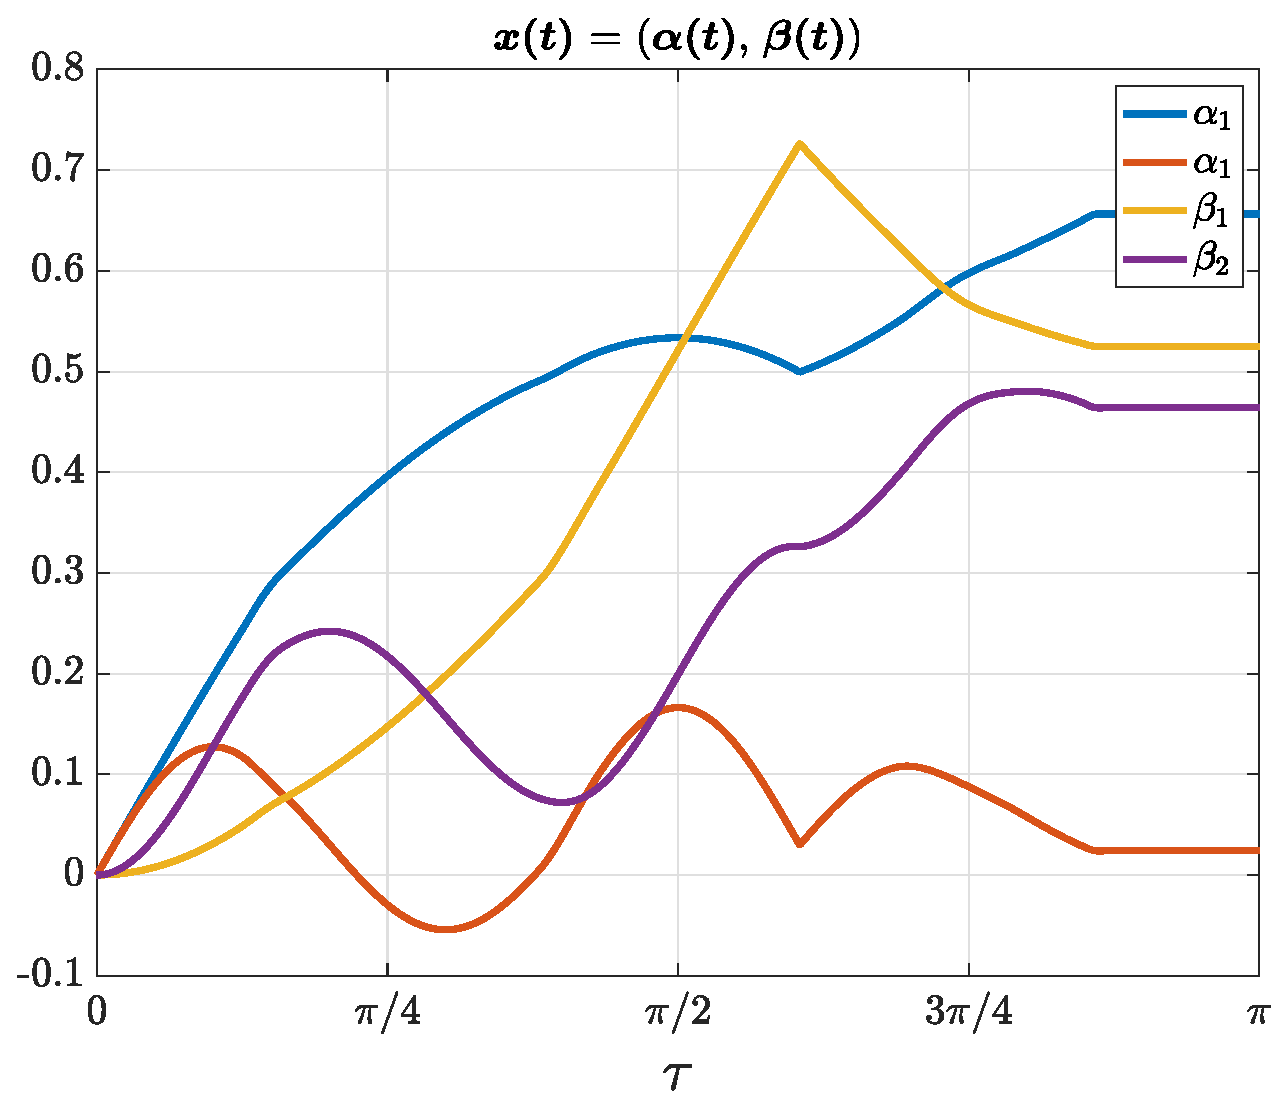
\includegraphics[scale=0.35]{img/fig02.eps}
	\caption{Evolución del sistema dinámico con los conjuntos $\mathcal{E}_a = \{1,2\}$ y $\mathcal{E}_b = \{1,2\}$ considerando el control $u(\tau)$ presentado en la figura \ref{fig:exampleSHE}}
\end{figure}

We can then formulate the following control problem, which is equivalent to Problem \ref{SHEp}:
\newline 
\begin{problem}\label{SHEpControl}
Let $\mathcal{U}$ be defined as in \eqref{eq:Udef} and let $\mathcal{E} _a $ and $\mathcal{E} _b $ be two sets of odd numbers with cardinalities $|\mathcal{E}_a| = N_a $ and $ |\mathcal{E} _b| = N_b$, respectively. Given the vectors $\bm{a}_T \in \mathbb{R}^{N_a}$ and $\bm{b}_T \in \mathbb{R}^{N_b} $, let us define $\bm{x}_T=[\bm{a}_T,\bm{b}_T]^\top \in \mathbb{R}^{N_a\times N_b}$. We look for $u:\in [0,\pi)\to\mathcal{U}$ such that the solution of \eqref{eq:CauchyReversed} with initial datum $\bm{x}(0)=\bm{x}_T$ satisfies $\bm{x}(\pi)=0$.
\end{problem}
$\newline$
\begin{remark}[Quarter-wave symmetry]
We shall mention that, in the SHE literature, it is usual to distinguish among the half-wave symmetry problem (addressed in the present paper) and the quarter-wave symmetry one in which
\begin{align*}
	u\left(\tau + \frac \pi2\right) = -u(\tau)\quad \mbox{for all}\; \tau \in \left[0,\frac \pi2\right).
\end{align*}
In quarter-wave symmetry, the SHE problem simplifies, as the Fourier coefficients $\{a_i\}_{i\in\mathcal E_a}$ turn out to be all zero. Hence, only the phases of the converter's signal can be controlled, while the half-wave SHE allows to deal with the amplitudes as well. It is worth to remark nonetheless that our optimal control formulation can be easily adapted to the quarter-wave symmetry problem by simply replacing the Fourier coefficients \eqref{eq:an} with
\begin{align*}
	a_i = 0, \quad\quad b_j = \frac{4}{\pi} \int_0^{\frac \pi4} u(\tau)  \sin(j \tau)\,d\tau.
\end{align*}
\end{remark}

